\section{Conclusion}\label{sec:conclusion}

Figure~\ref{fig:chain} shows how our findings fit together, from the job position to the knowledge it requires.

\begin{figure}[p]
\centering
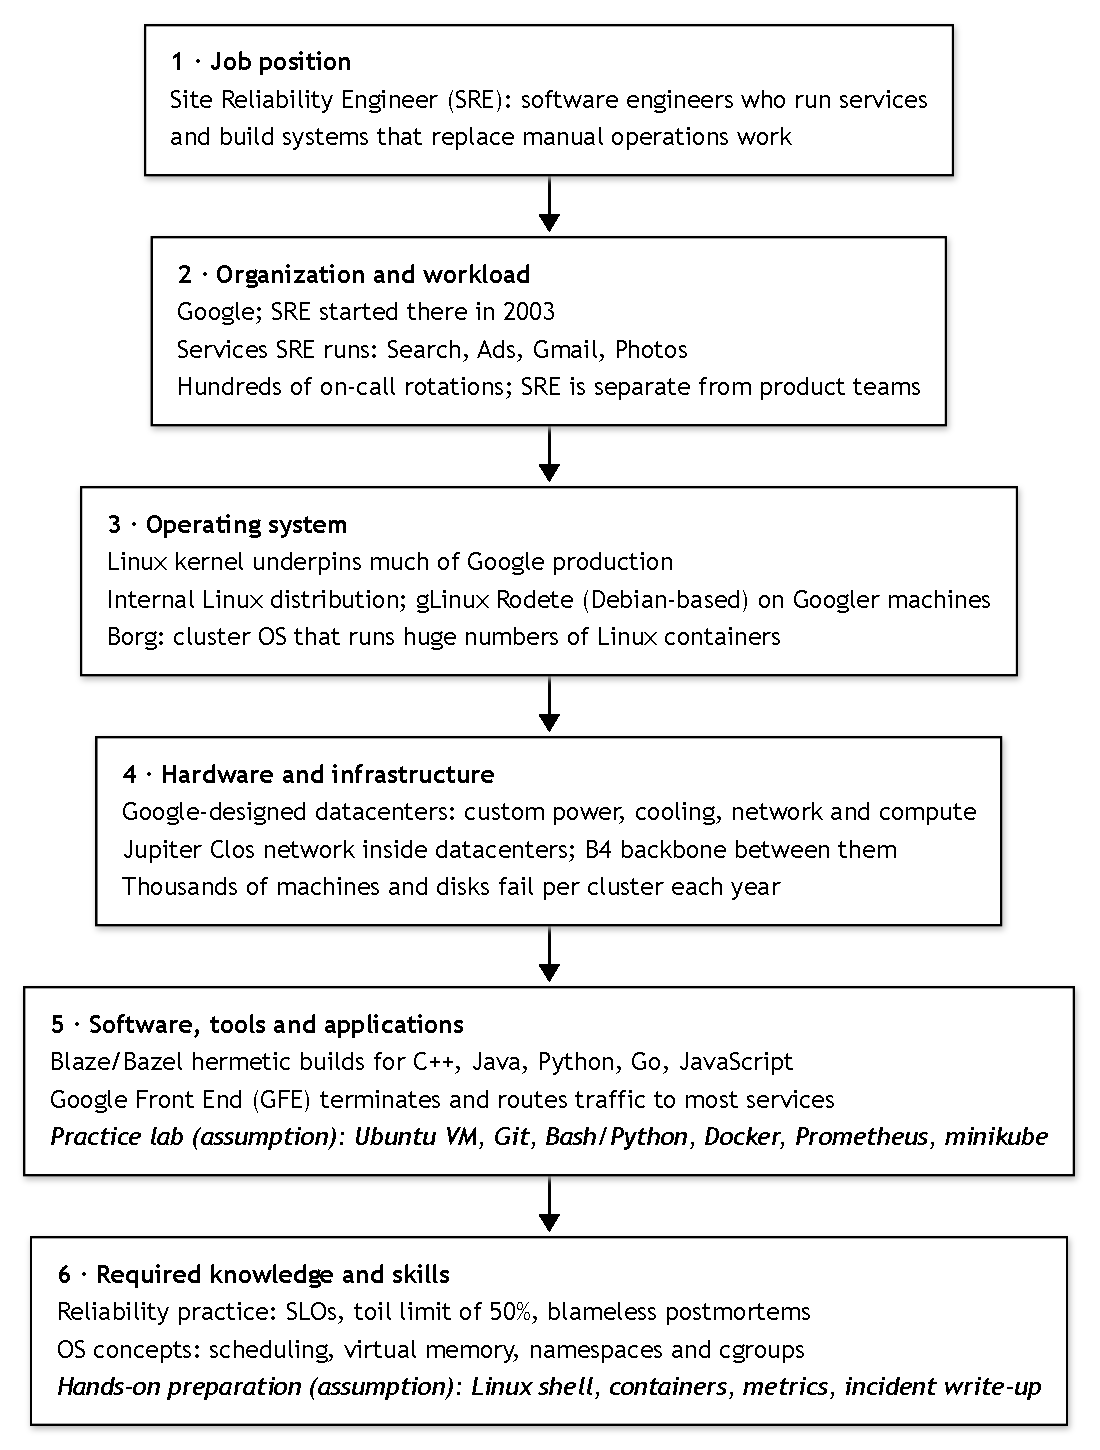
\includegraphics[width=0.94\textwidth,height=0.78\textheight,keepaspectratio]{figures/relationship.pdf}
\caption{From job position to required knowledge and skills for an SRE at Google. Each stage rests on human-verified claims from the cited sources \cite{sre-book,workbook,bsrs,cloud-google-blog-topics-developers-practitioners-how-google-got-to-rolling-linux-releases-for-desktops,static-pdf-incidentmanagementguide-pdf,man7-linux-man-pages-man7-sched-7-html,man7-linux-man-pages-man2-mmap-2-html,man7-linux-man-pages-man7-namespaces-7-html,docs-kernel-admin-guide-cgroup-v2-html}. The arrows read: works at, runs on, sits on top of, is operated with, requires. The two italic lines are our assumptions, a typical practice environment and a preparation recommendation, not verified facts about Google. The link from the OS concepts to the job is our interpretation.}
\label{fig:chain}
\end{figure}

\paragraph{What we found.}
At Google, SRE means software engineers who run services and build systems to replace manual operations work, with operational work limited to 50\% of a team's time \cite{sre-book,workbook}. The work runs on Linux: the kernel underpins much of Google's production infrastructure \cite{bsrs}, and Borg, the cluster operating system, runs huge numbers of Linux containers \cite{sre-book,workbook}. It runs in Google-designed datacenters where thousands of machines and disks fail in a typical year in one cluster \cite{sre-book}. Containers rely on Linux namespaces and control groups and share one kernel \cite{man7-linux-man-pages-man7-namespaces-7-html,docs-kernel-admin-guide-cgroup-v2-html,docs-docker-get-started-docker-concepts-the-basics-what-is-a-container}. In our reading, this links the job to process management, scheduling, virtual memory and resource control, but that link is our interpretation. The SRE book names UNIX system internals and networking (Layer 1 to Layer 3) as the two most common alternate technical skills it seeks \cite{sre-book}.

\paragraph{What we could not find.}
In the sources we read, we found no statement of which operating system Google SREs use on their own workstations. We found no description of an SRE internship program, its eligibility, locations or how to apply. We found no company history, revenue or customer counts beyond the examples in the SRE books, and no list of which CI/CD tools Google SRE uses now. We also found no source on projects given to student SREs. These gaps are noted where they arise. Anything about Google's internal environment that no source states is labelled as an assumption.

\paragraph{Reflection.}
GenAI sped up reading and organising sources, but it made mistakes that human review had to catch. We kept Generative AI output only where a source and a human check supported it.
